\documentclass[11pt,a4paper]{article}
\usepackage[utf8]{inputenc}
\usepackage[a4paper,margin=2.4cm]{geometry}
\usepackage{booktabs,array,graphicx,amsmath,xcolor,enumitem,url,caption}
\usepackage[hidelinks]{hyperref}
\captionsetup{font=small,labelfont=bf,skip=4pt}
\setlist{itemsep=1pt,topsep=3pt}
\setlength{\parskip}{3pt}

% ---- Fill in before submitting -------------------------------------------------
\newcommand{\authorname}{Pablo Mart\'in Perdomo}
\newcommand{\authordni}{78823396G}
\newcommand{\repourl}{\url{https://github.com/Pancrasi0/Big-Data-Individual-Assignment-II}}
% --------------------------------------------------------------------------------

\title{\textbf{Loop Order, Cache Blocking and CSR Storage in Sequential Java\\ Matrix Multiplication: A Controlled Measurement Study}\\[4pt]
\large Individual Assignment 2 --- Optimised Matrix Multiplication Approaches and Sparse Matrices}
\author{\authorname\ (DNI \authordni)\\ Subject: Big Data --- Grado en Ciencia e Ingenier\'ia de Datos, ULPGC \\ Academic year 2026--2027}
\date{October 2026}

\begin{document}
\maketitle

\begin{abstract}
We study two questions for sequential, double-precision $n\times n$ matrix multiplication in Java 21 on one desktop CPU: (A) how loop reordering and cache blocking change the runtime of a textbook triple loop, and (B) at which tested sparsity levels a self-implemented CSR (Gustavson) product beats dense multiplication, once conversion and output density are accounted for. Every configuration was measured with 2 warm-up and 5 timed repetitions in a fresh JVM, and every product was verified. Reordering the loops to \texttt{ikj} gave a 2.0--3.2$\times$ speedup over the baseline for $n\le 2500$. Blocked \texttt{ikj} was slower than plain \texttt{ikj} in 28 of 30 configurations; in 26 of them its throughput stayed near 2.5~GFLOP/s independently of $n$ and block size. CSR multiplication was faster than the best dense method in all 12 tested cases (sparsity 90--99.9\,\%, $n=1000$--$4000$): 8--23\,245$\times$ for the kernel alone and 7--723$\times$ including conversion. At 90--95\,\% sparsity the product $C$ was almost completely dense, which limited the gain, and at 99.9\,\% conversion accounted for about 98\,\% of the end-to-end time. The conclusions are limited to this implementation, JVM, hardware, and uniformly random nonzeros.
\end{abstract}

\section{Introduction and objective}
Matrix multiplication is the standard benchmark for studying how memory access patterns and data representations affect performance. This report builds on the basic dense algorithm and investigates two research questions:
\begin{itemize}
\item \textbf{RQ-A (dense optimisation).} How much do loop reordering and cache blocking improve the runtime of the textbook \texttt{ijk} triple loop as $n$ grows?
\item \textbf{RQ-B (sparse matrices).} For which tested sparsity levels does a CSR sparse--sparse product outperform dense multiplication, and how do conversion, indexing and output fill-in change the advantage?
\end{itemize}
The factors changed are the algorithm variant, $n$, the block size, and the sparsity; the outcomes are time per multiplication and memory. The \emph{predictions} made before the measurements, which the results either support or reject, were:
\begin{description}[leftmargin=1.6em,labelwidth=1.6em,labelsep=0.4em]
\item[H1] \texttt{ikj} is faster than \texttt{ijk}, and the gap grows once the matrices exceed the cache capacity.
\item[H2] Blocking gives a further gain over \texttt{ikj} for large $n$.
\item[H3] CSR is faster than dense multiplication at the tested sparsities, with a larger gain at higher sparsity.
\item[H4] The product becomes much denser than the inputs at low sparsity, reducing the advantage of CSR, and conversion cost matters when the multiplication itself is very cheap.
\end{description}

\section{Background}
\paragraph{Loop order and caches.} With row-major storage, the inner loop of \texttt{ijk} reads $B$ with stride $n$ (one new cache line per iteration), whereas \texttt{ikj} reads rows of $B$ and $C$ with stride 1, which is friendly to cache lines and hardware prefetching; this matters because memory access, not arithmetic, dominates \cite{drepper2007}. Both perform exactly $n^3$ multiply--adds, and here in the same summation order for each output element. \emph{Blocking} (tiling) restructures the loops to work on small sub-blocks so that data is reused while it is still in cache \cite{lam1991,goto2008}.
\paragraph{CSR and Gustavson's algorithm.} Compressed Sparse Row stores a matrix in three arrays: row pointers, column indices and values \cite{saad2003}. Gustavson's row-wise algorithm computes row $i$ of $C$ as the sum of the rows of $B$ selected by the nonzeros of row $i$ of $A$, using a dense accumulator \cite{gustavson1978}. Its work is proportional to the number of scalar products, about $\mathrm{nnz}(A)\,\mathrm{nnz}(B)/n$ for uniformly distributed nonzeros, plus per-row overhead; the output size is not known in advance.
\paragraph{Output fill-in.} If nonzeros are placed independently with densities $d_A$ and $d_B$, an entry of $C$ is nonzero with probability about $1-(1-d_Ad_B)^n$. This is used in Section~\ref{sec:nnz} as a check of the observed $\mathrm{nnz}(C)$.

\section{Methodology}
\subsection{Implementations}
All code is written for this study in Java (no external libraries, no library multiplication). Matrices are flat row-major \texttt{double[]} arrays, with element $(i,j)$ at index $in+j$.
\begin{center}\small
\begin{tabular}{@{}lp{10.2cm}@{}}\toprule
Method & Description\\\midrule
\texttt{ijk\_baseline} & Textbook triple loop, accumulating in a local variable, one store per $C_{ij}$.\\
\texttt{ikj\_reorder} & Loop order $i$-$k$-$j$ with $A_{ik}$ held in a register. \textbf{Change:} inner loop has stride 1 over $B$ and $C$. Expected effect: fewer cache misses, same arithmetic.\\
\texttt{blocked\_ikj} & \texttt{ikj} applied inside $bs\times bs$ tiles in the order $ii$-$kk$-$jj$; $bs\in\{32,64,128\}$; tile edges handled for any $n$. Expected effect: reuse of $B$ and $C$ tiles in cache.\\
\texttt{csr\_gustavson} & Own CSR (\texttt{rowPtr}, \texttt{colIdx}, \texttt{values}) and sparse--sparse Gustavson product with a dense accumulator and a marker array; output columns sorted per row; output arrays grow geometrically and are trimmed.\\\bottomrule
\end{tabular}
\end{center}
The baseline is the textbook algorithm re-implemented for this harness. The Java implementation of Assignment~1 used \texttt{int[][]} matrices with an \texttt{int} accumulator; here the matrices are flat \texttt{double[]} arrays with a 64-bit \texttt{double} accumulator, so the storage layout and numeric type differ and absolute times are not comparable with Assignment~1. All dense kernels write the full output (zero-fill inside \texttt{ikj} and blocked), so the three variants are compared with the same timing boundary.

\subsection{Inputs}
Inputs are generated with \texttt{java.util.Random}, whose algorithm is fixed by the Java specification; seed 42 for $A$ and 43 for $B$. Nonzero values are uniform in $[1,2)$ and \texttt{double} (64-bit) is the only numeric type. Part~A uses fully dense matrices. In Part~B, each position is nonzero independently with probability equal to the density, i.e.\ a uniform random nonzero distribution without structure; \emph{sparsity} is the percentage of zero entries and \emph{density} the percentage of nonzero entries. Realised $\mathrm{nnz}(A)$, $\mathrm{nnz}(B)$ and $\mathrm{nnz}(C)$ are recorded for every case. The same logical matrices (same seeds) are used by CSR and by the dense comparators of Part~B.

\subsection{Environment}
\begin{center}\small
\begin{tabular}{@{}ll@{}}\toprule
CPU & Intel Core i5-10400F @ 2.90~GHz (base), 6 physical cores, 12 logical processors\\
Cache & 12~MB shared L3 (Intel specification for this model; not measured in this study)\\
RAM & 16\,569\,368\,576 bytes (15.4~GiB)\\
OS & Linux 7.3.0-4 (CachyOS), amd64\\
JVM & OpenJDK 64-Bit Server VM 21.0.12.1 (Arch Linux build), default tiered JIT\\
JVM flags & \texttt{-Xms10g -Xmx10g -XX:+UseParallelGC}\\
Compiler & \texttt{javac -d out} (default options)\\
CPU governor & \texttt{performance}\\
Other load & Only a terminal; no other heavy programs running\\
Threads & Single-threaded kernels (12 logical processors visible to the JVM; none used for computation)\\\bottomrule
\end{tabular}
\end{center}
Fixed throughout: JDK, JVM flags, heap size, \texttt{double} type, seeds, value range, 2 warm-ups and 5 repetitions, and the time and memory budgets. An earlier launch of the experiment was interrupted because the machine went into suspend; its output was deleted and the study was rerun from an empty results directory (the final run was not interrupted).

\subsection{Timing boundary}
The timer is \texttt{System.nanoTime()} (monotonic). Inputs are generated, and the dense output array allocated, \emph{outside} the timed region. Three boundaries are used in Part~B and are never mixed in one comparison:
\begin{enumerate}[label=(\roman*)]
\item \textbf{kernel}: dense multiplication (including output zero-fill), or CSR multiplication of already converted matrices (including allocation and growth of the CSR output arrays);
\item \textbf{conversion}: dense $\to$ CSR for both $A$ and $B$, measured on its own;
\item \textbf{end-to-end}: conversion of $A$ and $B$ followed by the CSR multiplication, measured as one task starting from the dense inputs.
\end{enumerate}
Dense comparators need no conversion, so dense kernel time is compared with CSR kernel time (boundary i) and with CSR end-to-end time (boundary iii) separately. Results are consumed through a checksum computed after the timer stops, so the JIT compiler cannot discard the work \cite{georges2007}.

\subsection{Repetitions and statistics}
Each configuration runs in its own fresh JVM, runs the 266 self-tests (Section~\ref{sec:correct}), performs 2 warm-up executions of the measured task at full size (recorded in the raw CSV with \texttt{phase=warmup} and excluded from all statistics) and then 5 measured repetitions. I report the median and the interquartile range (IQR, linear interpolation); with only 5 samples the IQR is a coarse measure, so minimum and maximum are also kept in the summary files. Throughput is computed as $2n^3/t$ GFLOP/s, counting one multiplication and one addition per inner iteration. All raw samples are kept.

\subsection{Memory metrics}
Three different quantities are reported and not treated as interchangeable. (1) \emph{Array storage}: $3\cdot 8n^2$ bytes for dense $A$, $B$, $C$; for CSR, $4(n+1)+12\,\mathrm{nnz}$ bytes per matrix, summed over $A$, $B$, $C$. (2) \emph{Live JVM heap}: \texttt{totalMemory}$-$\texttt{freeMemory} after three \texttt{System.gc()} calls with the matrices still reachable; it also contains the dense inputs that the sparse JVM must hold for conversion and verification. (3) \emph{Peak resident set size} of the whole JVM process (\texttt{VmHWM} in \texttt{/proc/self/status}), which includes JVM runtime and garbage-collector effects.

\subsection{Correctness checks}\label{sec:correct}
Before every benchmark the program runs 266 tests and aborts on failure: a hand-computed $2\times2$ product; identity and zero matrices; random products for $n\in\{1,2,5,17,64,70\}$ against an independent \texttt{double[][]} reference, including block sizes 1, 7, 16 and 64 (not multiples of $n$); CSR round trips; sparse products at densities 1, 5, 10, 50 and 100\,\% against the dense reference, including equality of nnz and sorted column indices; and tests that the verification routine accepts a correct and rejects a corrupted product. Two values $x,y$ are considered equal if $|x-y|\le 10^{-12}+10^{-9}\max(|x|,|y|)$. Different evaluation orders change rounding only by a few units in the last place, so $10^{-9}$ relative leaves a wide margin, while indexing errors produce errors of order one. At benchmark sizes a full reference product would cost as much as the benchmark, so each result is checked with Freivalds' randomised test \cite{freivalds1977} ($Cx=A(Bx)$ for two random vectors, $O(n^2)$): all 80 verification records are \texttt{PASS}. In addition, the checksum of the product was bitwise identical across all dense methods and the CSR method for every $n$ (and sparsity), as expected since all methods add the products of each output element in ascending $k$ order.

\subsection{Size sequence and budgets}
Dense sizes: $n\in\{100,200,400,800,1200,1600,2000,2500,3000,4000\}$; sparse sizes $n\in\{1000,2000,4000\}$ with sparsity $\{90,95,99,99.9\}\,\%$; block sizes 32, 64, 128. Budgets declared in advance: at most 240~s per multiplication and an estimated 8192~MB per configuration (also capped at 85\,\% of the 10~GB heap). To limit total experiment time, the baseline \texttt{ijk} was not run for $n>2500$; this is a protocol cap, not a budget failure (Section~\ref{sec:limits}).

\section{Results}
\subsection{Part A: dense optimisation}
Table~\ref{tab:dense} and Fig.~\ref{fig:dense} show the runtime. The IQR is below 1.1\,\% of the median in every configuration, so repetitions within one process are very stable.

\begin{table}[t]\centering\small
\caption{Dense multiplication, median time in ms (IQR in ms). ``blk'' = blocked \texttt{ikj} with the given block size; 5 repetitions each; -- = not run.}\label{tab:dense}
\begin{tabular}{@{}rrrrrr@{}}\toprule
$n$ & ijk & ikj & blk 32 & blk 64 & blk 128\\\midrule
100 & 0.94 (0.00062) & 0.46 (0.0031) & 0.64 (0.0067) & 0.79 (0.00065) & 0.81 (0.0042) \\
200 & 8.01 (0.00048) & 3.75 (0.0043) & 6.47 (0.0014) & 6.29 (0.0094) & 6.34 (0.009) \\
400 & 67.3 (0.022) & 30.7 (0.004) & 51.5 (0.016) & 49.9 (0.019) & 51.4 (0.065) \\
800 & 543 (1.2) & 241 (0.59) & 411 (0.16) & 399 (0.17) & 239 (0.098) \\
1200 & 2\,490 (1.6) & 868 (4.1) & 1\,402 (1.5) & 1\,031 (0.16) & 1\,389 (0.12) \\
1600 & 8\,115 (33) & 2\,558 (3.7) & 3\,333 (0.55) & 3\,213 (1.1) & 3\,285 (0.19) \\
2000 & 15\,010 (14) & 5\,172 (3.6) & 6\,494 (1.5) & 6\,257 (0.54) & 6\,444 (0.61) \\
2500 & 30\,480 (13) & 9\,900 (5.6) & 12\,755 (0.86) & 12\,195 (0.59) & 12\,551 (1.1) \\
3000 & -- & 17\,088 (40) & 21\,883 (85) & 21\,059 (0.26) & 21\,818 (0.9) \\
4000 & -- & 42\,949 (26) & 51\,859 (1.4) & 38\,187 (3) & 51\,472 (1.3) \\\\\bottomrule
\end{tabular}
\end{table}

\begin{figure}[t]\centering
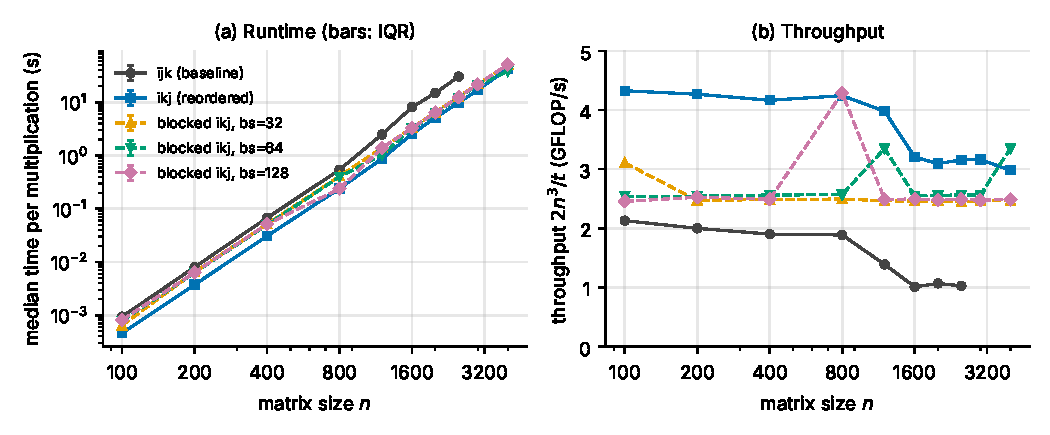
\includegraphics[width=\textwidth]{figs/fig_dense.pdf}
\caption{Dense multiplication. (a) Median time per multiplication (log--log; bars: IQR, mostly smaller than the markers). (b) Throughput $2n^3/t$.}\label{fig:dense}
\end{figure}

\begin{table}[t]\centering\small
\caption{Speedup of the median time, relative to \texttt{ijk} (left, only where \texttt{ijk} was run) and relative to \texttt{ikj} (right). Values below 1 mean slower.}\label{tab:speedup}
\begin{tabular}{@{}r|rrrr|rrr@{}}\toprule
 & \multicolumn{4}{c|}{vs.\ \texttt{ijk}} & \multicolumn{3}{c}{blocked vs.\ \texttt{ikj}}\\
$n$ & ikj & blk 32 & blk 64 & blk 128 & blk 32 & blk 64 & blk 128\\\midrule
100 & 2.03 & 1.46 & 1.19 & 1.15 & 0.72 & 0.59 & 0.57 \\
200 & 2.14 & 1.24 & 1.27 & 1.26 & 0.58 & 0.60 & 0.59 \\
400 & 2.19 & 1.31 & 1.35 & 1.31 & 0.60 & 0.62 & 0.60 \\
800 & 2.25 & 1.32 & 1.36 & 2.27 & 0.59 & 0.61 & 1.01 \\
1200 & 2.87 & 1.78 & 2.41 & 1.79 & 0.62 & 0.84 & 0.63 \\
1600 & 3.17 & 2.43 & 2.53 & 2.47 & 0.77 & 0.80 & 0.78 \\
2000 & 2.90 & 2.31 & 2.40 & 2.33 & 0.80 & 0.83 & 0.80 \\
2500 & 3.08 & 2.39 & 2.50 & 2.43 & 0.78 & 0.81 & 0.79 \\
3000 & -- & -- & -- & -- & 0.78 & 0.81 & 0.78 \\
4000 & -- & -- & -- & -- & 0.83 & 1.12 & 0.83 \\\\\bottomrule
\end{tabular}
\end{table}

\paragraph{Reordering (H1).} \texttt{ikj} was 2.0--2.3$\times$ faster than \texttt{ijk} for $n\le 800$ and 2.9--3.2$\times$ for $n\ge 1200$. Throughput of \texttt{ijk} fell from 2.1 to about 1.0~GFLOP/s between $n=100$ and $n\ge1600$, whereas \texttt{ikj} fell from 4.3 to about 3.0--3.2~GFLOP/s.
\paragraph{Blocking (H2).} Blocked throughput was almost constant, 2.45--2.57~GFLOP/s, in 26 of the 30 configurations, with no systematic effect of the block size (32, 64, 128 within a few percent). Because \texttt{ikj} is faster for small $n$, blocked \texttt{ikj} was \emph{slower} than plain \texttt{ikj} (0.57--0.83$\times$ for $n\ge 100$ in these 26 configurations). Four configurations ran in a faster regime (3.1--4.3~GFLOP/s): bs=32 at $n=100$ (0.72$\times$ relative to \texttt{ikj}), bs=128 at $n=800$ (1.01$\times$), bs=64 at $n=1200$ (0.84$\times$) and bs=64 at $n=4000$ (1.12$\times$). The last is the only configuration where blocking was clearly faster than \texttt{ikj}: 38.2~s against 42.9~s, while bs=32 and bs=128 took 51.9 and 51.5~s at the same size.
\paragraph{Growth with $n$.} An ordinary least-squares fit of $\log t$ on $\log n$ for $n\ge1600$ gives exponents of 2.97 (\texttt{ijk}), 3.06 (\texttt{ikj}), 3.00 (blocked, bs=32 and 128) and 2.74 for bs=64 (affected by the fast $n=4000$ point). Over the whole range the exponents are 3.25 (\texttt{ijk}) and 3.11 (\texttt{ikj}); the excess over 3 for \texttt{ijk} comes from the drop in throughput between $n=800$ and $n=1600$ (Table~\ref{tab:dense}).

\subsection{Part B: sparse CSR versus dense}
\begin{table}[t]\centering\footnotesize
\caption{Sparse versus dense (median time in seconds). $S_\text{mul}$ and $S_\text{e2e}$: time of dense \texttt{ikj} divided by the CSR kernel time and by the CSR end-to-end time (conversion included). Sparsity in \%; nnz are realised counts; ``dens.\ $C$'' = density of $C$ in \%.}\label{tab:sparse}
\setlength{\tabcolsep}{3.2pt}
\resizebox{\textwidth}{!}{%
\begin{tabular}{@{}rrrrr|r|rrr|rr@{}}\toprule
$n$ & sp. & nnz($A$) & nnz($C$) & dens.\ $C$ & dense ikj & CSR mul. & conv. & CSR e2e & $S_\text{mul}$ & $S_\text{e2e}$\\\midrule
1000 & 90 & 99\,941 & 999\,959 & 100.00 & 0.466 & 0.059 & 0.0053 & 0.064 & 8.0 & 7.3 \\
1000 & 95 & 49\,819 & 917\,311 & 91.73 & 0.556 & 0.045 & 0.0042 & 0.049 & 12.5 & 11.4 \\
1000 & 99 & 9\,927 & 94\,238 & 9.42 & 0.473 & 0.0042 & 0.0036 & 0.0068 & 113 & 69.0 \\
1000 & 99.9 & 981 & 953 & 0.10 & 0.475 & 0.0001 & 0.0035 & 0.0036 & 4\,214 & 134 \\
\midrule
2000 & 90 & 399\,687 & 4\,000\,000 & 100.00 & 4.99 & 0.302 & 0.021 & 0.322 & 16.5 & 15.5 \\
2000 & 95 & 199\,626 & 3\,972\,763 & 99.32 & 4.99 & 0.207 & 0.017 & 0.224 & 24.2 & 22.3 \\
2000 & 99 & 39\,717 & 716\,586 & 17.91 & 5.17 & 0.027 & 0.015 & 0.042 & 193 & 124 \\
2000 & 99.9 & 3\,961 & 7\,880 & 0.20 & 5.17 & 0.0004 & 0.014 & 0.014 & 12\,631 & 373 \\
\midrule
4000 & 90 & 1\,599\,452 & 16\,000\,000 & 100.00 & 40.71 & 1.99 & 0.083 & 2.04 & 20.5 & 20.0 \\
4000 & 95 & 799\,382 & 15\,999\,259 & 100.00 & 42.71 & 1.03 & 0.069 & 1.09 & 41.7 & 39.1 \\
4000 & 99 & 159\,899 & 5\,265\,110 & 32.91 & 40.64 & 0.218 & 0.057 & 0.276 & 187 & 147 \\
4000 & 99.9 & 16\,004 & 63\,327 & 0.40 & 40.73 & 0.0018 & 0.055 & 0.056 & 23\,245 & 723 \\\\\bottomrule
\end{tabular}}
\end{table}

\begin{figure}[t]\centering
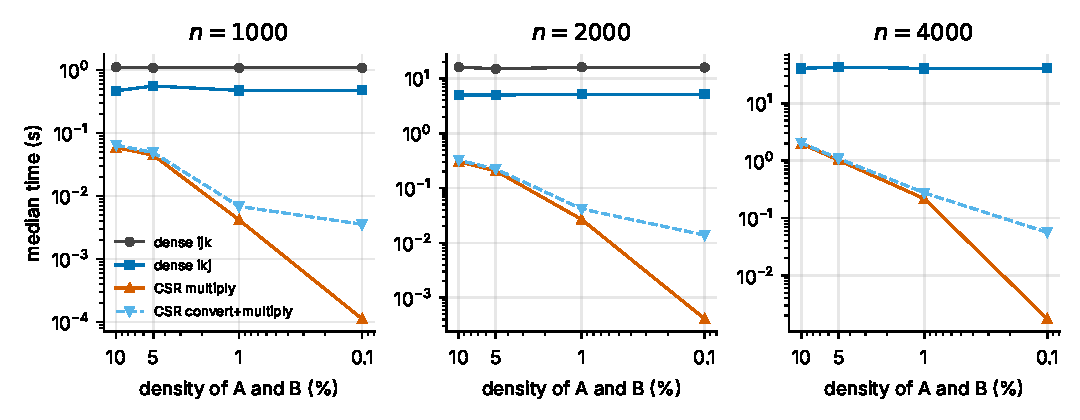
\includegraphics[width=\textwidth]{figs/fig_sparse_time.pdf}
\caption{Median time versus density of the inputs (the axis is reversed: sparser to the right). Dense \texttt{ijk} was not run at $n=4000$.}\label{fig:sparse}
\end{figure}

Table~\ref{tab:sparse} and Fig.~\ref{fig:sparse} summarise the comparison. Dense times do not depend on sparsity, as expected, since the dense kernels perform the same work on zeros.
\paragraph{Where CSR helps (H3).} CSR was faster than the best dense method (\texttt{ikj}) in all 12 cases, and the gain grew with sparsity: $S_\text{mul}$ is 8.0--20.5$\times$ at 90\,\%, 12.5--41.7$\times$ at 95\,\%, 113--193$\times$ at 99\,\% and 4\,214--23\,245$\times$ at 99.9\,\%. The gain also increased with $n$ at fixed sparsity (except between $n=2000$ and $4000$ at 99\,\%). No crossover was observed because the tested range starts at 90\,\% sparsity. For $n=1000$ and 2000, where \texttt{ijk} was also run, the ratios against \texttt{ijk} would be 2.3--3.2$\times$ larger; that part is an optimisation effect and is discussed separately in Section~\ref{sec:disc}.
\paragraph{Conversion (H4).} Converting $A$ and $B$ took 3.5--5.3~ms ($n=1000$), 14--21~ms ($n=2000$) and 55--83~ms ($n=4000$): it scales as $n^2$ (about $4\times$ per doubling) and decreases moderately with sparsity, since fewer nonzeros are stored. At 90\,\% sparsity it is only 4\,\% of the end-to-end time ($n=4000$), but at 99.9\,\% it is 98\,\% (55~ms of 56~ms), so $S_\text{e2e}$ drops from 23\,245$\times$ (kernel) to 723$\times$ (end-to-end). Whether conversion is included therefore changes the 99.9\,\% speedup by a factor of 32 at $n=4000$.
\paragraph{Per-operation cost.} The speedup is smaller than the ideal ratio of operation counts ($1/d^2$) because a CSR product is more expensive than a dense multiply--add. Table~\ref{tab:cost} compares the estimated cost per scalar product of the CSR kernel with the cost per multiply--add of dense \texttt{ikj}: CSR costs 3--123~ns per product against 0.47--0.67~ns, i.e.\ 4.9--260$\times$ more. The ratio is lowest for the largest $n$ and densest inputs and large when there are few products (99.9\,\%), where fixed per-call and per-row work (allocating and clearing the accumulator, sorting, trimming) dominates. The experiments do not isolate which of these contributes most.

\begin{table}[t]\centering\small
\caption{Estimated cost per scalar operation. Products of the CSR kernel are estimated as $\mathrm{nnz}(A)\,\mathrm{nnz}(B)/n$ (exact in expectation for uniform nonzeros, not counted directly); the dense cost is $t/n^3$ for \texttt{ikj}.}\label{tab:cost}
\begin{tabular}{@{}rrrrrr@{}}\toprule
$n$ & sparsity (\%) & products ($10^6$) & CSR ns/product & dense ns/madd & ratio\\\midrule
1000 & 90 & 9.982 & 5.87 & 0.47 & 12.6 \\
1000 & 95 & 2.487 & 17.90 & 0.56 & 32.2 \\
1000 & 99 & 0.098 & 42.41 & 0.47 & 89.7 \\
1000 & 99.9 & 0.001 & 123.19 & 0.47 & 259.5 \\
\midrule
2000 & 90 & 79.746 & 3.78 & 0.62 & 6.1 \\
2000 & 95 & 19.940 & 10.37 & 0.62 & 16.6 \\
2000 & 99 & 0.789 & 33.88 & 0.65 & 52.4 \\
2000 & 99.9 & 0.008 & 52.03 & 0.65 & 80.5 \\
\midrule
4000 & 90 & 638.944 & 3.11 & 0.64 & 4.9 \\
4000 & 95 & 159.582 & 6.42 & 0.67 & 9.6 \\
4000 & 99 & 6.379 & 34.16 & 0.63 & 53.8 \\
4000 & 99.9 & 0.064 & 27.49 & 0.64 & 43.2 \\\\\bottomrule
\end{tabular}
\end{table}

\subsection{Nonzeros of the product}\label{sec:nnz}
\begin{figure}[t]\centering
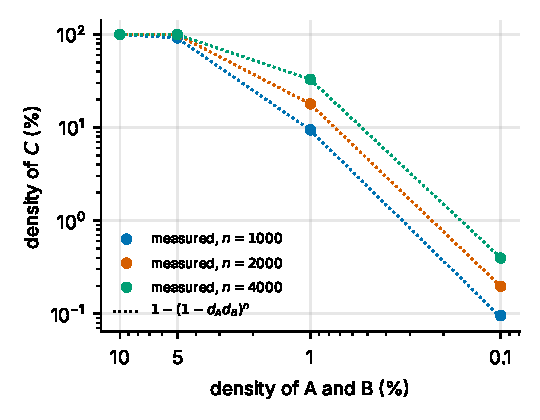
\includegraphics[width=0.49\textwidth]{figs/fig_nnz.pdf}\hfill
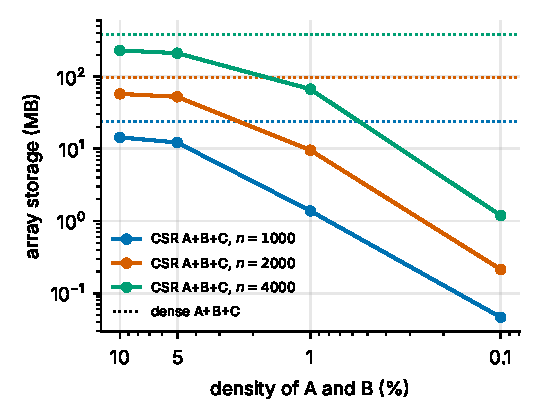
\includegraphics[width=0.49\textwidth]{figs/fig_mem.pdf}
\caption{Left: measured density of $C$ versus the model $1-(1-d_Ad_B)^n$ (dotted). Right: array storage of CSR $A$+$B$+$C$ versus dense $A$+$B$+$C$ (dotted lines).}\label{fig:nnzmem}
\end{figure}
The product is far denser than the inputs when the inputs are not very sparse: $\mathrm{nnz}(C)/\mathrm{nnz}(A)$ was 10--20 at 90--95\,\%, up to 33 at 99\,\% and 1.0--4.0 at 99.9\,\%. At 90\,\% sparsity $C$ is 99.996--100\,\% dense for every $n$, and at 95\,\% it is 91.7\,\% ($n=1000$) to 99.99\,\% ($n=4000$) dense. The probabilistic model of Section~2 reproduces the measured density of $C$ to within 0.6\,\% (relative) in 11 of 12 cases (e.g.\ 32.88\,\% predicted versus 32.91\,\% measured at $n=4000$, 99\,\%) and 4\,\% in the remaining one ($n=1000$, 99.9\,\%: 953 nonzeros measured, about 914 predicted). So in these experiments the output cost is largely predictable from the inputs' density, but only for uniformly random nonzeros.

\subsection{Memory}
\begin{table}[t]\centering\small
\caption{Dense memory (\texttt{ikj}; for the other methods the RSS is within 2\,\% and the live heap within 0.2~MB). MB = $10^6$ bytes.}\label{tab:densemem}
\begin{tabular}{@{}rrrr@{}}\toprule
$n$ & array storage $3\cdot8n^2$ & live heap after GC & peak RSS\\\midrule
100 & 0.2 & 1.7 & 133 \\
200 & 1.0 & 2.4 & 134 \\
400 & 3.8 & 5.3 & 138 \\
800 & 15.4 & 16.8 & 169 \\
1200 & 34.6 & 36.0 & 225 \\
1600 & 61.4 & 62.9 & 309 \\
2000 & 96.0 & 97.4 & 409 \\
2500 & 150.0 & 151.4 & 578 \\
3000 & 216.0 & 217.4 & 785 \\
4000 & 384.0 & 385.4 & 1296 \\\\\bottomrule
\end{tabular}
\end{table}
For dense matrices the live heap equals the array storage plus a constant of about 1.4~MB, as expected. Peak RSS is much larger (1.30~GB at $n=4000$, 3.4$\times$ the arrays) because it also includes the JVM runtime and garbage-collector copying; I did not instrument the collector to attribute it.

\begin{table}[t]\centering\small
\caption{Memory in Part~B. Array storage of CSR $A$+$B$+$C$ versus dense $A$+$B$+$C$ ($24n^2$ bytes), and peak RSS of the JVM that ran the CSR kernel versus the JVM that ran dense \texttt{ikj} (MB = $10^6$ bytes).}\label{tab:sparsemem}
\begin{tabular}{@{}rrrrrrr@{}}\toprule
$n$ & sparsity (\%) & CSR (MB) & dense (MB) & CSR/dense (\%) & RSS CSR (MB) & RSS dense (MB)\\\midrule
1000 & 90 & 14.41 & 24 & 60.0 & 903 & 195 \\
1000 & 95 & 12.22 & 24 & 50.9 & 888 & 195 \\
1000 & 99 & 1.38 & 24 & 5.8 & 234 & 196 \\
1000 & 99.9 & 0.05 & 24 & 0.2 & 176 & 194 \\
\midrule
2000 & 90 & 57.61 & 96 & 60.0 & 3059 & 410 \\
2000 & 95 & 52.49 & 96 & 54.7 & 3057 & 409 \\
2000 & 99 & 9.58 & 96 & 10.0 & 836 & 410 \\
2000 & 99.9 & 0.21 & 96 & 0.2 & 326 & 407 \\
\midrule
4000 & 90 & 230.42 & 384 & 60.0 & 4301 & 1298 \\
4000 & 95 & 211.21 & 384 & 55.0 & 4137 & 1296 \\
4000 & 99 & 67.06 & 384 & 17.5 & 3525 & 1294 \\
4000 & 99.9 & 1.19 & 384 & 0.3 & 940 & 1296 \\\\\bottomrule
\end{tabular}
\end{table}
For the CSR representation, array storage is 60\,\% of the dense storage at 90\,\% sparsity, 51--55\,\% at 95\,\% (the saving comes from $A$ and $B$, because $C$ is almost dense and 12 bytes per nonzero in CSR exceed the 8 bytes of a dense entry), 6--17\,\% at 99\,\% and below 0.4\,\% at 99.9\,\%. The increment of live heap caused by the CSR objects equals the storage estimate to within 30~kB. In contrast, the peak RSS of the CSR JVM is higher than that of the dense JVM at $n=4000$ in 90--99\,\% sparsity (up to 4.3~GB against 1.3~GB): that JVM also holds the dense inputs needed for conversion and verification, and the geometric growth of the output arrays creates garbage. RSS therefore must not be read as the memory cost of the CSR format itself.

\subsection{Limits and budgets}\label{sec:limits}
No configuration exceeded the declared budgets: no timeouts, no memory failures and no skipped configuration because of a budget (\texttt{summary\_limits.csv} contains no entries). The largest \emph{tested} size that satisfied the limits was $n=4000$ for all dense methods other than \texttt{ijk} and for CSR (slowest multiplication: 51.9~s versus the 240~s budget; largest estimated memory 384~MB versus 8192~MB). The largest \emph{attempted} size was also 4000, so these are the limits of the declared size sequence, not the limits of the machine. The baseline \texttt{ijk} was tested up to $n=2500$ (30.5~s) only; extrapolating the measured $O(n^3)$ trend suggests that $n=3000$ and 4000 would also fit in the time budget, but this is an extrapolation, not a measurement. Consequently, Part~B has no \texttt{ijk} comparator at $n=4000$.

\section{Discussion}\label{sec:disc}
\paragraph{Answer to RQ-A.} H1 is supported: loop reordering alone gave a 2.0--3.2$\times$ speedup with no extra memory and no change in arithmetic. The throughput curves are consistent with an access-pattern explanation: with the vendor-specified 12~MB L3, the matrix $B$ is 5.1~MB at $n=800$, 11.5~MB at $n=1200$ and 20.5~MB at $n=1600$, and the \texttt{ijk} throughput falls in steps (1.9, 1.4, 1.0~GFLOP/s) as $B$ grows towards and beyond that capacity, while the stride-1 \texttt{ikj} loop degrades much less (4.2, 4.0, 3.2). This is an inference from timing trends; I collected no hardware counters, so cache misses were not observed directly. H2 is not supported in the tested range: blocked versions were slower than \texttt{ikj} in 28 of 30 configurations (one tie at 1.01$\times$, bs=128, $n=800$) and only one configuration (bs=64, $n=4000$) was clearly faster. Blocking did make the throughput independent of $n$ (flat 2.5~GFLOP/s), which indicates that it removes the size-dependent cache penalty, but at a lower level than \texttt{ikj} reaches for small $n$; the narrowing ratio (bs=32: 0.60 at $n=400$, 0.83 at $n=4000$) suggests that a crossover for the slow regime might lie beyond the tested sizes, which remains untested. Plausible causes for the lower plateau, which I did not test, are the loop overhead of short inner loops (32--128 iterations) and different code generation by the JIT; the absence of any effect of the block size supports the view that cache capacity is not what limits the blocked code here.
\paragraph{Variability between JVM launches.} The four ``fast regime'' blocked results, with throughputs of up to 4.3~GFLOP/s (similar to \texttt{ikj}), cannot be explained by the within-process IQR, which is below 1.1\,\% everywhere. Because each configuration ran in its own JVM, between-process differences (JIT decisions, memory placement) are not captured by the IQR. The dense comparators of Part~B give a direct estimate: they perform identical work for all sparsity levels, yet their medians vary by up to 19\,\% (\texttt{ikj}, $n=1000$: 0.466--0.556~s), 3.7\,\% ($n=2000$) and 5.1\,\% ($n=4000$); for \texttt{ijk}, 2.6\,\% ($n=1000$) and 7.3\,\% ($n=2000$). The blocked kernels showed even larger jumps (up to 1.7$\times$) between configurations that perform the same work, so individual blocked-versus-\texttt{ikj} comparisons are less certain than the 4--7\,\% spread of the dense comparators at large $n$ suggests. The 2--3$\times$ differences between \texttt{ijk} and \texttt{ikj}, and the sparse speedups of one to four orders of magnitude, are far outside all these ranges.
\paragraph{Optimisation versus sparse storage.} The two effects were measured separately. The optimisation effect (\texttt{ijk}$\to$\texttt{ikj}) is a constant-factor change of 2--3$\times$ on dense data. The sparse effect is of a different kind: CSR reduces the \emph{number} of operations to roughly $d^2n^3$, but each operation costs 5--260$\times$ more (Table~\ref{tab:cost}), so the net gain is $1/(d^2\rho)$ with the cost ratio $\rho$. If $\rho$ stayed at the 5--13 measured at 90\,\% sparsity, break-even would occur around 28--45\,\% density (55--72\,\% sparsity); this extrapolation lies outside the tested range, and $\rho$ itself changes with density, so it is a hypothesis for a follow-up experiment with sparsity 50--85\,\%, not a result.
\paragraph{Where the sparse advantage shrinks.} Three effects reduce it, and they act in different regimes: (i) fill-in at 90--95\,\% sparsity (the output is practically dense, so CSR pays indexing overhead and 12~bytes per entry for a result that a dense array stores in 8); (ii) the higher per-operation cost of indexing and accumulation; (iii) conversion from dense at very high sparsity, where the multiplication is cheap and the $O(n^2)$ conversion dominates. If the sparse matrices were created and kept in CSR form, (iii) would disappear, but (i) and (ii) would remain.
\paragraph{Limitations.}
\begin{itemize}
\item One machine, one JDK and one JIT: conclusions about \texttt{ikj}/blocked/CSR are not statements about Java or any language in general.
\item Five repetitions per process and one process per configuration; between-process variability is only estimated indirectly (above).
\item No hardware counters or JIT logs, so cache and code-generation explanations are inferences consistent with the data.
\item Sparsity only from 90\,\% to 99.9\,\% and only uniformly random nonzeros; structured matrices (banded, block, power-law) can behave differently, and a percentage of zeros alone does not determine performance.
\item Only one sparse algorithm and format (CSR/Gustavson, sorted output) and three block sizes; unrolling, SIMD and other formats were not studied. The number of scalar products in Table~\ref{tab:cost} is estimated, not counted.
\item \texttt{ijk} was not run for $n>2500$ (protocol cap).
\end{itemize}

\section{Conclusions}
Within the tested scope (sequential Java~21, double precision, one i5-10400F, sizes up to $n=4000$, uniformly random nonzeros): (1) loop reordering from \texttt{ijk} to \texttt{ikj} was the most effective dense optimisation, with a 2.0--3.2$\times$ speedup that grows as $B$ exceeds the cache; (2) blocking made the throughput independent of $n$ but was slower than \texttt{ikj} in 28 of 30 configurations, and the few faster configurations show that single results depend on the JVM run; (3) CSR was faster than the best dense method in every tested case, from 7$\times$ (90\,\% sparsity, end-to-end) to over 23\,000$\times$ (99.9\,\%, kernel only); (4) the advantage is reduced by output fill-in, by a per-operation cost 5--260 times that of the dense kernel, and, at very high sparsity, by the conversion, which accounted for 98\,\% of the end-to-end time; (5) the nonzero count of the product matched a simple independence model within 0.6\,\% in 11 of 12 cases. Unresolved: the sparsity at which dense multiplication overtakes CSR, the cause of the blocked plateau and of the fast-regime outliers (hardware counters and repeated JVM launches are needed), and behaviour on structured sparse inputs.

\section*{References and materials}
\renewcommand{\refname}{\vspace{-1.2em}}
\begin{thebibliography}{9}\small
\bibitem{goto2008} K.~Goto and R.~A. van de Geijn, ``Anatomy of high-performance matrix multiplication,'' \emph{ACM Trans. Math. Softw.}, vol.~34, no.~3, pp.~12:1--12:25, 2008.
\bibitem{lam1991} M.~D. Lam, E.~E. Rothberg, and M.~E. Wolf, ``The cache performance and optimizations of blocked algorithms,'' in \emph{Proc. 4th Int. Conf. Architectural Support for Programming Languages and Operating Systems (ASPLOS IV)}, 1991, pp.~63--74.
\bibitem{gustavson1978} F.~G. Gustavson, ``Two fast algorithms for sparse matrices: Multiplication and permuted transposition,'' \emph{ACM Trans. Math. Softw.}, vol.~4, no.~3, pp.~250--269, 1978.
\bibitem{saad2003} Y.~Saad, \emph{Iterative Methods for Sparse Linear Systems}, 2nd ed. Philadelphia, PA: SIAM, 2003.
\bibitem{freivalds1977} R.~Freivalds, ``Probabilistic machines can use less running time,'' in \emph{Information Processing 77 (Proc. IFIP Congress 1977)}. Amsterdam: North-Holland, 1977, pp.~839--842.
\bibitem{georges2007} A.~Georges, D.~Buytaert, and L.~Eeckhout, ``Statistically rigorous Java performance evaluation,'' in \emph{Proc. 22nd ACM SIGPLAN Conf. Object-Oriented Programming, Systems, Languages and Applications (OOPSLA)}, 2007, pp.~57--76.
\bibitem{drepper2007} U.~Drepper, ``What every programmer should know about memory,'' Red Hat, Inc., Nov.\ 2007.
\bibitem{course2026} ``BIG DATA --- Individual Assignments: Matrix Multiplication, revised proposal 2026--2027,'' Universidad de Las Palmas de Gran Canaria, 2026.
\end{thebibliography}

\paragraph{Reproducibility materials.} All materials are in the public repository \repourl: the Java source code, a README with the exact build and run commands, the raw measurements (900 records; columns: experiment, method, $n$, density, sparsity, seed, block size, numeric type, repetition, phase, time in ns, nonzero counts, memory metrics, checksum, verification, status), the environment file, the analysis script that produces the summaries and plots, and the script that generates the figures and tables of this report. Inputs are regenerated from the seeds; nothing needs to be downloaded. The whole study was run with a script that starts one fresh JVM per configuration; the console log is included. Note that the environment file is written by the first JVM only and therefore lists the configuration of that first launch; the parameters of the study are those given in this report.

\paragraph{Use of generative AI.} Generative AI (Claude, Anthropic) was used to accelerate the creation of the benchmarks and of all the measurement and analysis scripts, in order to build them as carefully as possible, and for a first draft of this report. I had already prepared my own design of the matrix generation and multiplication components, with a very similar structure; I adopted the AI-generated version because it added improvements to some of them. I reviewed the code, ran all experiments on my own machine, and am responsible for the measurements, the interpretation and the conclusions. Generated text is not treated as evidence.

\end{document}
